We assume that the stellar density profile follows a broken power law
with the stellar density $\rhostar\sim r^{-1-\Gamma}= r^{-\delta}$ inside of the
break radius $\rb$, where ($0<\Gamma<1$). We derive an expression for
the specific enthalpy of the gas, $\ke +\gammaf \frac{p}{\rho}$ as a
function of $\zeta=v_w/\sigma$, $x=r/r_s$, and $r_s/\rsoi$. We show
that if the break radius, $\rb$ goes to infinity this quantity
necessarily goes to infinity as the potential well becomes infinitely
deep, hence a break radius is necessary for an outflow to be possible.

Consider the steady state energy conservation equation. {\bf AG perhaps
  put a brief explanation of how this relates to the steady state
  entropy equation via laws of thermodynamics?.}

\begin{align}
\frac{1}{r^2} \frac{d}{dr} \left(r^2 \rho v \left(\frac{v^2}{2} + \Phi
    + \gammaf \frac{p}{\rho}\right) \right) = q \kew + q \Phi,
\label{eq:enCons}
\end{align}

Where $\vw^2=v_w^2+\sigma^2= v_w^2+\frac{3}{\Gamma+2}\frac{G
  \Mbh}{r}+\sigma_0^2$.

Now integrate both sides with respect from r to the stagnation radius 

\begin{align}
  r^2 \rho v \left(\ke+\Phi+\gammaf \frac{p}{\rho} \right)= \int_{\rs}^{r}
    r^2 \left(q \kew + q\Phi\right) dr
    \label{eq:enConsInt}
\end{align}

We know $f\equiv r^2 \rho v$ from the steady state mass conservation
equation. 

\begin{align}
 \frac{1}{r^2} \frac{d}{dr} \left(r^2 \rho v\right) = q 
\end{align}

Where q is the rate of the mass injection per volume, which is
proportional to the stellar density. Let $x=r/\rs$ and $q_o= q
(\rs)$. Then $q=q_o x^{-\delta}$. 

Then one obtains for the mass flux, $f=r^2 \rho v$,

\begin{align}
 f(x)=q_o \rs^3 \left[\frac{x^{3-\delta}-1}{3-\delta}\right].
 \label{eq:massFlux}
\end{align}

The gravitational potential $\Phi$ is given by

\begin{align}
\Phi&= -\frac{G \Menc}{r} - 4 \pi G \int_{r}^{\infty} \rhostar(r') r'
dr'.\nonumber\\
&\simeq -\frac{G \Menc}{r} -4 \pi G \int_{r}^{\rb} \rhostar(r') r' dr'
\label{eq:Phi}
\end{align}

Where in the scond line we have neglected the contribution of the
stars outside of the break radius, $\rb$, to the gravitational potential.

% Note our unconventional choice of gauge: the upper limit of the
% integral on the right hand side is $\rs$ whereas conventionally the
% upper limit is taken to be $\infty$. This means that our definition
% will not give $\Phi=0$ in the limit $r\rightarrow\infty$. However,
% our result for the enthalpy $\ke + \gammaf \frac{p}{\rho}$ will be
% gauge invariant. 

Using equations~\eqref{eq:enConsInt},~\eqref{eq:massFlux},
and~\eqref{eq:Phi}, we may obtain an expression for the Bernoulli
parameter of the gas, $\ke+\gammaf \frac{p}{\rho} +\Phi$ of the gas inside
of the break radius $\rb$.

\begin{align}
  &\frac{v^2}{2}+\gammaf \frac{p}{\rho} +\Phi = \nonumber\\
  &-U_o\left[\frac{\rs/\rb}{2-\delta}-\frac{x^{5-2\delta}-1}{x^{3-\delta}-1}\frac{3-\delta}{(5-2\delta)(2-\delta)}\right]\nonumber\\
  &+\frac{v_w^2}{2}+\frac{\sigma_0^2}{2}- \frac{G \Mbh}{r_s}
  \frac{1-2\delta}{2(\delta+1)} \frac{3-\delta}{2-\delta}\frac{x^{2-\delta}-1}{x^{3-\delta}-1}
  \nonumber\\
  &-\frac{G M_\star}{r_s}
  \frac{x^{5-2\delta}-1}{x^{3-\delta}-1}\frac{3-\delta}{5-2\delta},
\end{align}

where $U_o=4 \pi G \rhostar(\rs) \rs^2$.  We may rewrite this as 

\begin{multline}
  \frac{v^2}{2}+\gammaf \frac{p}{\rho}+\Phi
=\frac{G \Mbh}{\rs} 
\biggl[
  \frac{3}{2} \zeta^2 w^{\frac{1}{3 -\delta}}
  -\frac{(1-2\delta)(3-\delta)}{2(\delta+1)(2-\delta)}  \frac{x^{2  -\delta}-1}{x^{3-\delta}-1}\\
  -\frac{\rb}{\rsoi} w^{\frac{\delta-1}{3-\delta}} \frac{3 -\delta}{2 -\delta} 
  -w \frac{(2-\delta)(3-\delta)-(3-\delta)^{2}}{(5-2\delta)(2-\delta)} \frac{x^{5-2\delta}-1}{x^{3-\delta}-1}
\biggr].
\label{eq:enthAnal}
\end{multline}

Recall that $\rs$ the stagnation radius, $x\equiv r/\rs$, $\zeta=\sqrt{v_w^2+\sigma_0^2}/\sigma_0$, $w\equiv (\rs/\rsoi)^{3\delta}$, and
$\delta$ is the power law slope of the stellar density profile inside
of the break radius, $\rb$.

% For sufficiently large radii ($x$), the expression above always
% becomes negative, which means that a break in the stellar density
% profile is necessary in order to obtain an outflow.
 For a given $\rb/\rsoi$ there is a critical $\zeta$, $\zeta_{c}$, such
 that if $\zeta>\zeta_c$, an outflow will be possible from any
radius, since the Bernoulli parameter will be positive inside of the
break radius. On the other hand if $\zeta<\zeta_c$, then there is a
minimum value of $(\rs/\rsoi)_{\rm min}$. If we have had
$\rs/\rsoi<(\rs/\rsoi)_{\rm min}$, then the Bernoulli parameter would
become negative inside of $\rb$ and no outflow would be possible.

For cusp galaxies ($\Gamma$=0.8), $\zeta_c\simeq \sqrt 2$
($v_w\simeq\sigma_0$).  On the other hand for core galaxies
($\Gamma$=0.1) we find $\zeta_c\simeq (\rb/\rsoi)^{0.45}$, see the top
panel of Fig.~\ref{fig:zetaCrit}. For values of $\zeta<\zeta_c$, the
stagnation radius rapidly approaches the break radius as shown in the
bottom panel of Fig.~\ref{fig:zetaCrit}.
% We also find that for core galaxies for $\zeta<\zeta_c$, there is a minimum
% for $\rs/\rsoi$, $\left(\rs/\rsoi\right)_{\rm min}$--if $\rs/\rsoi$ were
% less than this value the gas enthalpy would become negative inside of
% the break radius which is clearly unphysical.  This may be roughly
% approximated using (see Fig.~\ref{fig:rbRinf})

% \begin{align}
% &\left.\frac{\rs}{\rsoi}\right|_{\rm min}=\frac{\rb}{\rsoi} \frac{\sqrt{\zeta_c-\zeta}}{\sqrt{\zeta_c-1}}\nonumber\\
% &\zeta_c\simeq \frac{\rb}{\rsoi}^{0.45}
% \label{eq:rsRinfCrit}
% \end{align}


\begin{figure}
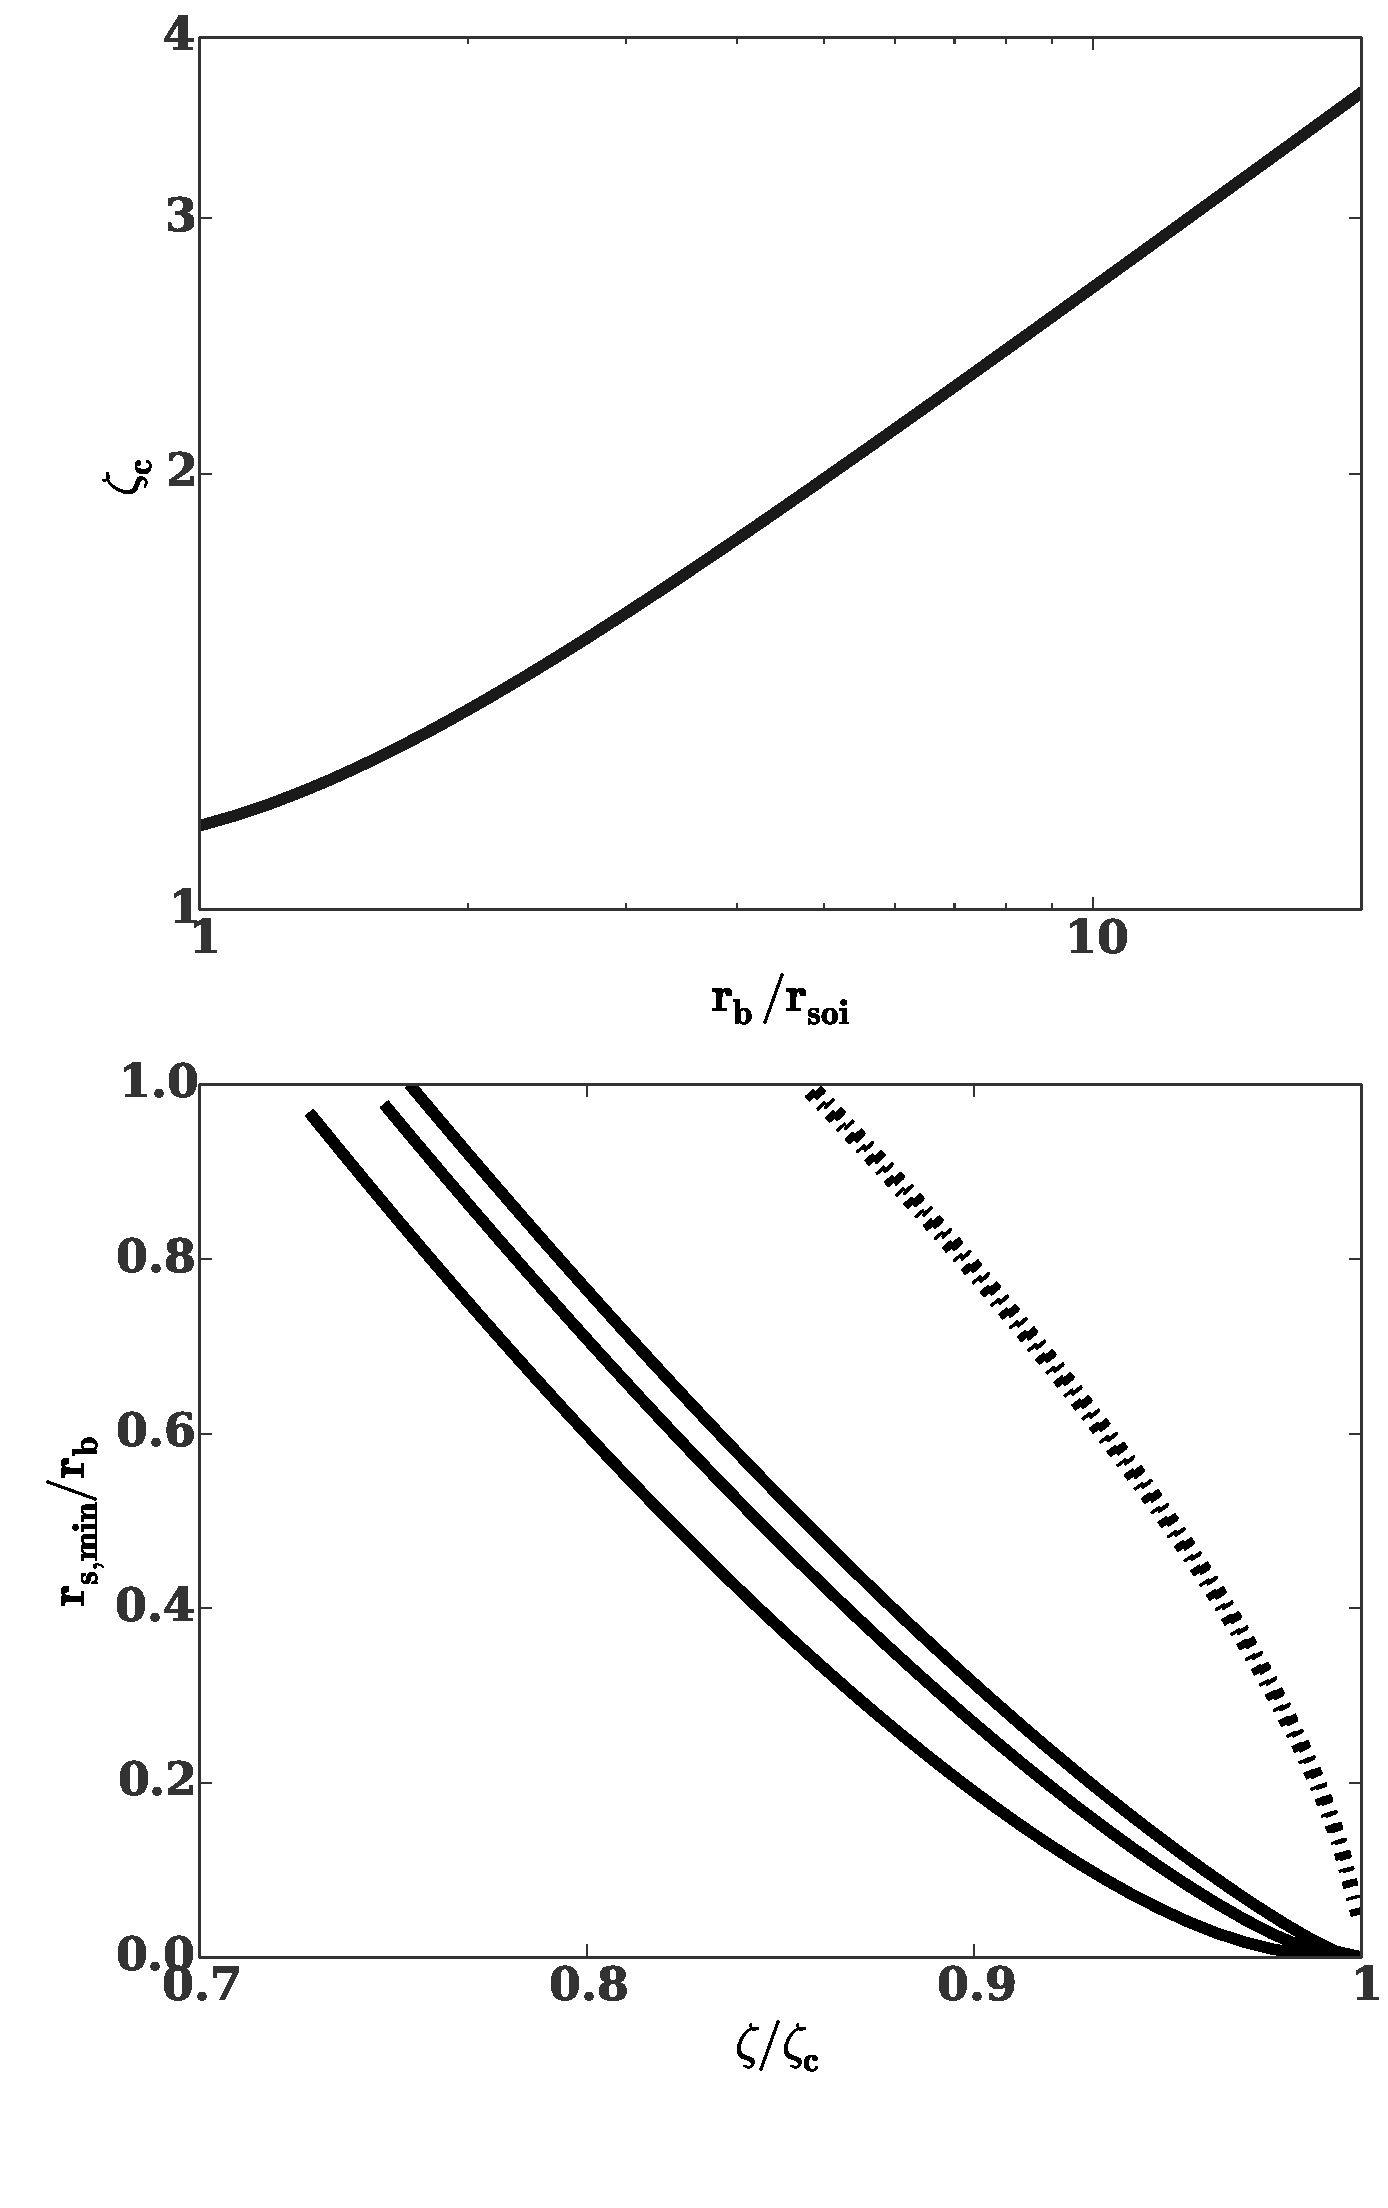
\includegraphics[width=\columnwidth]{zetaCrit.pdf}
\caption{\label{fig:zetaCrit} Mininmum value for ratio of the stagnation
  radius to the influence radius, $\rs/\rsoi$ for core galaxies
  ($\Gamma=0.1$) derived by requiring enthalpy of the gas to remain
  positive out to the break radius $\rb$. The solid lines correspond
  to the constraint computed numerically from
  equation~\eqref{eq:enthAnal}, while the dashed line correspond the
  results of the fitting formula equation~\eqref{eq:rsRinfCrit}. The
  x-intercept of each curve corresponds to the critical $\zeta$,
  $\zeta_c$ above which an outflow is possible from any radius}
\end{figure}


%%% Local Variables: 
%%% mode: latex
%%% TeX-master: "ms"
%%% End: 
